\section{Error analysis}
Our solution is to use 3D-CNN with VGG-like structure. We optimized cross-entropy loss and used MSE as a main metric. Another metric was accuracy on binarized target. 
We benchmark performance of our model against CatBoost regressor trained on physics and chemistry features extracted from data. 
The results are presented on the graphics as follows.
\begin{center}
\caption{Performance on train of CNN model}
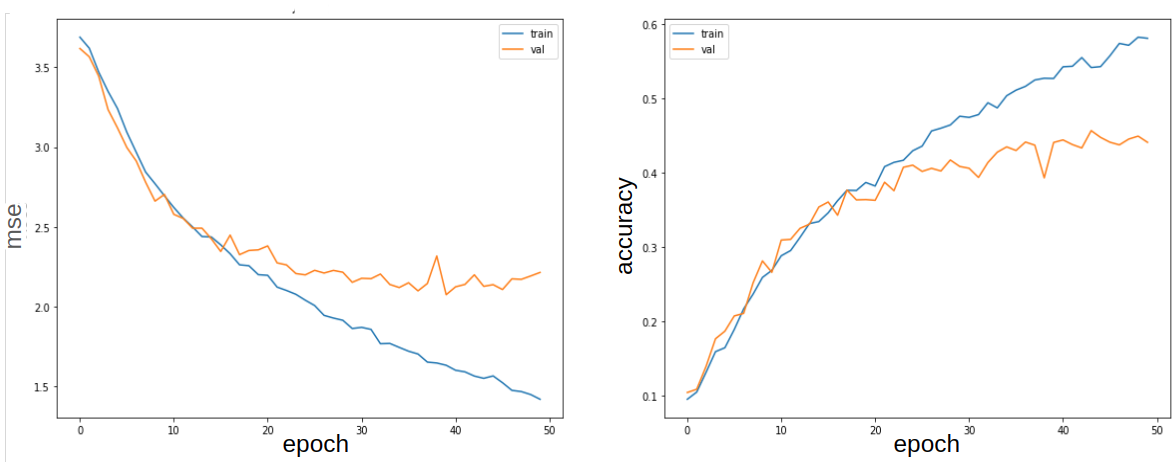
\includegraphics[width=0.8\textwidth]{contents/CNN_error.png}
\end{center}

\begin{tabular}{ |p{5cm}|p{5cm}|p{5cm}|  }
        \hline
        \multicolumn{3}{|c|}{Test metrics} \\
        \hline
        Model & MSE & Accuracy\\
        \hline
        3D-CNN, VGG based & 0.8715 & 0.72\\
        CatBoost on manual features & 1.2 & 0.53\\
        Basic Model & 4.8 & 0.172\\
        \hline
\end{tabular}

The performance of our present model is significantly better than the regressor on well-known features.